\chapter{Comparison with stochastic models}
\label{ch:models}

Chapters~\ref{ch:observables} and~\ref{ch:global} established displacement growth,
quantile behaviour, directional anisotropy and duration effects without assuming a
generating process.
This chapter confronts those measurements with explicit stochastic-process
predictions: the moment spectrum and a L\'evy-walk benchmark, centred kurtosis as
a shape diagnostic, velocity memory across averaging resolutions, and a summary
of which candidates the measurements challenge or leave open.

\section{The moment spectrum and the L\'evy-walk benchmark}
\label{sec:transport-shape}

For $q>0$, define a moment and its growth exponent by
\begin{equation}
  M_q(\tau)=\mathbb E[R(t,\tau)^q],\qquad
  M_q(\tau)\propto\tau^{\zeta(q)},\qquad \nu(q)=\zeta(q)/q.
  \label{eq:moment-spectrum}
\end{equation}
A common scaling law with finite moments gives $\zeta(q)=qH$. Increasing $q$ gives large
displacements more weight, so the spectrum tests a different aspect of the distribution
from any one quantile. Plain increments are used here: second differences of a straight
leg vanish and would change the physical observable being compared.

For an unbiased renewal L\'evy walk with independent isotropically chosen headings,
constant speed and leg-duration density
$\psi(t)\sim t^{-1-\beta}$, the superdiffusive regime $1<\beta<2$ predicts
\begin{equation}
  \zeta_{\mathrm{LW}}(q)=
  \begin{cases}
    q/\beta,&0<q<\beta,\\
    q+1-\beta,&q>\beta,
  \end{cases}
  \qquad \zeta_{\mathrm{LW}}(2)=3-\beta.
  \label{eq:levy-spectrum}
\end{equation}
At $q=\beta$ a logarithmic correction accompanies the common power. The bulk and the
rare long legs contribute different branches; their meeting produces strong anomalous
scaling~\cite{zaburdaev2015,rebenshtok2014}. This benchmark is an asymptotic model
prediction with stated renewal and speed assumptions.

\begin{figure}[htbp]
  \centering
  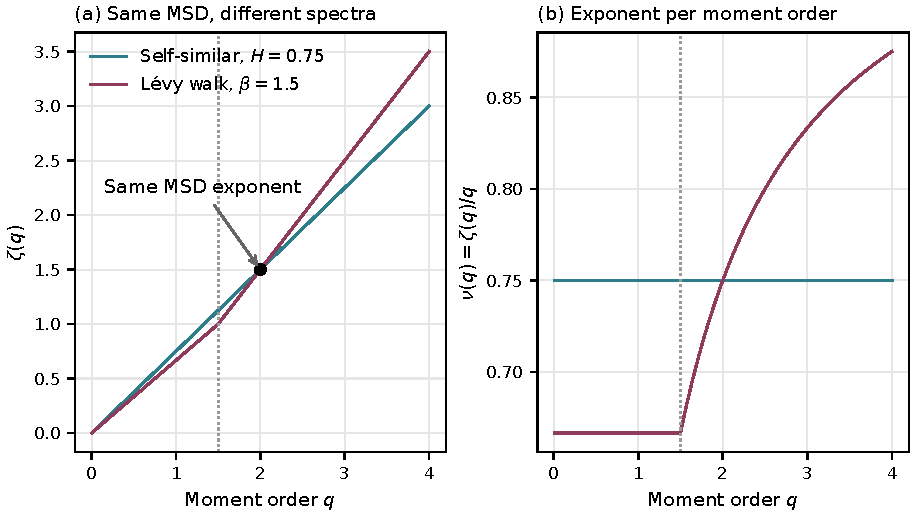
\includegraphics[width=\linewidth]{generated/moment_spectrum_schematic}
  \caption{Theoretical comparison. A self-similar process with $H=0.75$ and a standard
  L\'evy walk with $\beta=1.5$ have the same MSD exponent, $\zeta(2)=1.5$, but different
  moment spectra. The dashed vertical line marks $q=\beta$. These are asymptotic
  predictions, not simulated or empirical estimates.}
  \label{fig:levy-spectrum-schematic}
\end{figure}

Read per unit order, Eq.~\eqref{eq:levy-spectrum} predicts
\begin{equation}
  \nu_{\mathrm{LW}}(q)=\frac{\zeta_{\mathrm{LW}}(q)}{q}=
  \begin{cases}
    1/\beta,&0<q<\beta,\\[2pt]
    1-\dfrac{\beta-1}{q},&q>\beta,
  \end{cases}
  \label{eq:levy-spectrum-per-order}
\end{equation}
a spectrum that is flat below the knee and \emph{rises} above it towards the ballistic
value one. The benchmark fixes a level, a knee position and a direction of curvature at
once, which is more than the second moment alone can test.

\ifscalingresultsready
The measurement of Sec.~\ref{sec:moment-spectrum} curves the other way. On the fixed
population and over the reference window, $\nu$ falls monotonically from
\StatSSParaSpectrumNuLow\ to \StatSSParaSpectrumNuHigh\ in paragliders and from
\StatSSHangSpectrumNuLow\ to \StatSSHangSpectrumNuHigh\ in hang gliders, with paired
whole-flight intervals that exclude a flat spectrum
(Fig.~\ref{fig:fixed-spectrum}, Table~\ref{tab:spectrum}). Matching the second moment
alone would need $\beta=3-\zeta(2)=\StatSSParaSpectrumLevyBeta$ and
\StatSSHangSpectrumLevyBeta, and that choice predicts
$\nu\simeq1/\beta=\StatSSParaSpectrumLevyNu$ and \StatSSHangSpectrumLevyNu\ at low
order, below what is measured there, followed by a rise where the measurement declines.
No single $\beta$ in $(1,2)$ reproduces the level and the curvature together.

Figure~\ref{fig:shape} shows the same observable pooled over the population that
changes with lag. That spectrum rises with $q$ and so agrees with the benchmark in
direction. The disagreement between the two is a sampling effect rather than a
difference of observable, which is why the comparison above uses the controlled
measurement.

\else
The fixed-population spectrum and its paired bootstrap intervals are awaiting
regeneration (Sec.~\ref{sec:moment-spectrum}). Its comparison with the benchmark,
including any numerical estimate of $\beta$ and any claimed incompatibility of
curvature, remains pending. Figure~\ref{fig:shape} retains the available pooled
spectrum, whose contributing population changes with lag; it cannot substitute
for that controlled comparison.
\fi

A spectrum over one window cannot exclude every L\'evy walk or every possible
crossover. Ballistic L\'evy walks, truncated legs, correlated steps
and finite-time crossovers need separate predictions. A quantitative test requires
simulations with the observed durations, sampling and preprocessing, compared jointly
with moments and controlled quantiles. High-order moments also need flight-level
sensitivity checks; the 90th percentile alone need not track the ballistic front.

\begin{figure}[htbp]
  \centering
  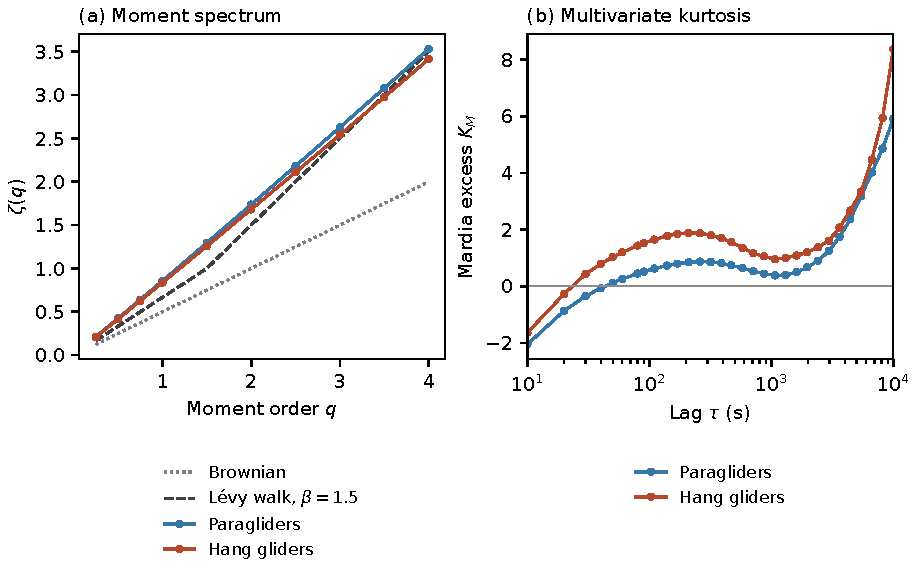
\includegraphics[width=\linewidth]{generated/ch3_models}
  \caption{Displacement moment spectra and centred multivariate kurtosis in the diagnostic
  eligible archive, with theoretical moment spectra shown as reference curves. These observables
  constrain the growth and shape of the increment distribution, respectively, but neither
  alone identifies the generating process. The contributing flights change with lag here,
  unlike the fixed cohort of Sec.~\ref{sec:quantile-population}: short flights leave the
  pool as $\tau$ grows, so part of the change along either curve is a change of
  population. These spectra are therefore read as archive descriptions; the
  \ifscalingresultsready
  fixed-population spectrum of Fig.~\ref{fig:fixed-spectrum} and the rank-resolved
  exponents of Sec.~\ref{sec:component-self-similarity} carry the self-similarity
  comparison.
  \else
  rank-resolved exponents of Sec.~\ref{sec:component-self-similarity} remain the
  available controlled measurements; the fixed-population spectrum is pending.
  \fi}
  \label{fig:shape}
\end{figure}

\section{Centred kurtosis and heterogeneity}
\label{sec:transport-gaussian}

At each lag with a finite, positive-definite covariance, centre the increment and
standardise by that full covariance:
\begin{equation}
  Q=(\mathbf X-\boldsymbol\mu)^\top\Sigma^{-1}(\mathbf X-\boldsymbol\mu),
  \qquad K_M(\tau)=\mathbb E[Q^2]-d(d+2),\quad d=2.
  \label{eq:nongauss}
\end{equation}
Mardia's kurtosis excess~\cite{mardia1970} vanishes for a nonsingular Gaussian
vector, including an anisotropic one, since $Q\sim\chi_d^2$. Positive excess
means a larger fourth moment of standardised radius. It neither requires a
power-law tail nor makes zero excess sufficient for Gaussianity.

For the $n$ pooled increments at a lag, the calculation uses
\begin{equation}
 \begin{aligned}
 \widehat{\boldsymbol\mu}&=\frac1n\sum_{i=1}^n\mathbf X_i,\qquad
 \widehat K_M=\frac1n\sum_{i=1}^n\widehat Q_i^2-8,
 \\
 \widehat\Sigma&=\frac1n\sum_{i=1}^n
  (\mathbf X_i-\widehat{\boldsymbol\mu})
  (\mathbf X_i-\widehat{\boldsymbol\mu})^\top.
 \end{aligned}
 \label{eq:empirical-mardia}
\end{equation}
Here $\widehat Q_i$ uses these empirical moments. With covariance denominator $n$,
$n^{-1}\sum_i\widehat Q_i=2$, so Jensen's inequality gives
$\widehat K_M\ge-4$. Negative excess is possible, and even a Gaussian sample
need not give exactly zero.

The measured $K_M$ is not constant. Across the displayed interval its range is
\StatRevParaMardiaMin\ to \StatRevParaMardiaMax\ for paragliders and
\StatRevHangMardiaMin\ to \StatRevHangMardiaMax\ for hang gliders. The medians over
sampled lags are \StatRevParaMardiaMedian\ and \StatRevHangMardiaMedian, respectively;
these lag medians are descriptive summaries, not time averages. The change of sign near
the shortest lags and the rise where support is smallest discourage replacing the curve
with one claim about a tail.

Excess can also arise from heterogeneity even when the conditional motion is Gaussian.
For example, let $\mathbf X=\sqrt A\,\mathbf G$, where $\mathbf G$ is a centred Gaussian vector with
fixed covariance, $A>0$ is independent, and both required moments exist. Then
\begin{equation}
  K_M=d(d+2)\left[\frac{\mathbb E A^2}{(\mathbb E A)^2}-1\right].
  \label{eq:pooled-nongauss}
\end{equation}
This identity applies to the stated scale mixture; flights with different means
and covariance orientations require a fuller calculation. The pooled excess
therefore compares the archive with one homogeneous Gaussian law. Conditional
Gaussian models need separate centring and covariance estimates within environment
or phase groups, with simulations accounting for finite samples and dependence.
A peak in pooled kurtosis alone cannot identify a thermal timescale.

\section{Velocity memory across resolutions}
\label{sec:transport-memory}

A fix-to-fix velocity mixes recorder cadence, smoothing and physical turning. To examine
longer scales, define velocity averaged over a duration $h$,
\begin{equation}
  \mathbf v_h(t)=\frac{\mathbf r(t+h)-\mathbf r(t)}{h},\qquad
  C_h(\tau)=\frac{\langle\delta\mathbf v_h(t)\cdot
                             \delta\mathbf v_h(t+\tau)\rangle}
                         {\langle|\delta\mathbf v_h|^2\rangle}.
  \label{eq:vacf}
\end{equation}
We compare $h=10$, $60$ and \SI{300}{\second}. In each retained segment $fs$,
form $n_{fs}$ adjacent velocity blocks and subtract their segment mean.
The segment estimate and archive average are
\begin{equation}
\begin{aligned}
 \widehat C_{fs,h}(kh)
 &=\frac{(n_{fs}-k)^{-1}\sum_{j=0}^{n_{fs}-k-1}
       \delta\mathbf v_{fs,j}\cdot\delta\mathbf v_{fs,j+k}}
      {n_{fs}^{-1}\sum_{j=0}^{n_{fs}-1}|\delta\mathbf v_{fs,j}|^2},\\[4pt]
 \widehat C_h(kh)
 &=\frac1{|\mathcal F_h(k)|}\sum_{f\in\mathcal F_h(k)}
   \frac1{|\mathcal S_{f,h}(k)|}\sum_{s\in\mathcal S_{f,h}(k)}\widehat C_{fs,h}(kh).
\end{aligned}
\label{eq:vacf-estimator}
\end{equation}
Here $\mathcal S_{f,h}(k)$ contains the supported segments of flight $f$:
\[
 n_{fs}\ge8,\qquad
 \sum_j|\delta\mathbf v_{fs,j}|^2>0,\qquad
 1\le k\le\lfloor n_{fs}/4\rfloor.
\]
Flights with a nonempty set form $\mathcal F_h(k)$. Segments receive equal weight
within each flight, then flights receive equal weight. This differs from normalising
one pooled covariance.

The separation $\tau=kh\ge h$ avoids overlap between the two velocity blocks.
Finite-segment centring can nevertheless depress long-lag correlations.

Figure~\ref{fig:velocity-memory} places the positive correlations on logarithmic axes,
where a power-law interval would satisfy
\begin{equation}
 C_h(\tau)\simeq A_h\tau^{-\gamma_h}
 \quad\Longrightarrow\quad
 \log C_h(\tau)\simeq\log A_h-\gamma_h\log\tau.
 \label{eq:vacf-loglaw}
\end{equation}
The linear-ordinate panels retain zero crossings and negative correlation.

\begin{figure}[!htbp]
 \centering
 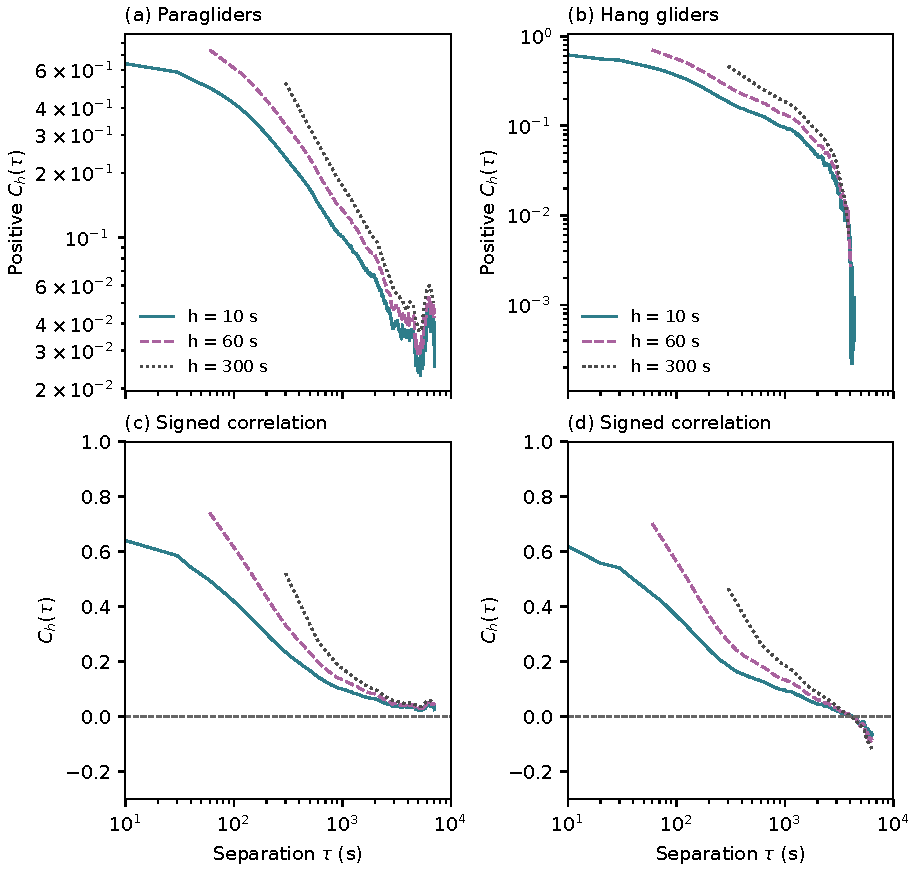
\includegraphics[width=\linewidth]{generated/ch3_velocity_memory}
 \caption{Velocity memory at averaging widths $h=10$, $60$ and $\SI{300}{\second}$.
 The upper panels use log--log axes for positive correlations; nonpositive values interrupt
 the curves. The lower panels show the same estimates with a linear vertical axis,
 preserving zero crossings and anticorrelation. At least 20 contributing flights are
 required, with separation no shorter than $h$ and no longer than one quarter of each
 contributing velocity record. The contributing flights change with separation, so a
 slope read from these curves mixes decaying memory with the loss of short records.
 A visually straight part of the upper curves is a possible scaling interval; it is
 not evidence of an asymptotic law.}
 \label{fig:velocity-memory}
\end{figure}

\FloatBarrier
At a ten-minute separation, all three resolutions retain positive sample means:
\begin{center}
\begin{tabular}{@{}rcc@{}}
\toprule
\textbf{Width $h$ [s]} & \textbf{Paraglider $\widehat C_h(600\,\mathrm s)$}
 & \textbf{Hang-glider $\widehat C_h(600\,\mathrm s)$} \\
\midrule
10 & \StatRevParaVacfTenAtSixHundred & \StatRevHangVacfTenAtSixHundred \\
60 & \StatRevParaVacfSixtyAtSixHundred & \StatRevHangVacfSixtyAtSixHundred \\
300 & \StatRevParaVacfThreeHundredAtSixHundred & \StatRevHangVacfThreeHundredAtSixHundred \\
\bottomrule
\end{tabular}
\end{center}
No calibrated intervals are reported here. Coarse averaging suppresses fast
fluctuations and can increase normalized correlation without lengthening the
underlying memory. The log--log curves bend, and estimates in both disciplines
turn negative at long separation; one decay exponent does not describe the full interval.

\paragraph{Memory and displacement growth.}

For a stationary centred velocity with variance
$\sigma_v^2=\langle|\delta\mathbf v|^2\rangle$, integrating velocity over the
displacement interval and using stationarity gives Taylor's relation~\cite{taylor1922},
\begin{equation}
  M_{2,c}(\tau)=2\sigma_v^2\int_0^\tau(\tau-s)C(s)\,\mathrm ds.
  \label{eq:green-kubo}
\end{equation}
The factor $\sigma_v^2$ restores the velocity units because $C$ is normalised.
Taylor's relation concerns centred displacement in the same stationary population.

For example, an exponentially correlated velocity, $C(s)=e^{-s/t_p}$, gives
\begin{equation}
  M_{2,c}(\tau)=2\sigma_v^2t_p
      \left[\tau-t_p(1-e^{-\tau/t_p})\right].
  \label{eq:persistent-msd}
\end{equation}
Its limits are
\[
 M_{2,c}(\tau)\simeq
 \begin{cases}
  \sigma_v^2\tau^2, & \tau\ll t_p \quad\text{(ballistic)},\\
  2\sigma_v^2t_p\tau, & \tau\gg t_p \quad\text{(diffusive)}.
 \end{cases}
\]
An intermediate superdiffusive slope can therefore arise from finite persistence.
Different $t_p$ across flights broaden the crossover. A fitted MSD slope above
one does not exclude this model.

An asymptotic tail $C(s)\sim s^{-\gamma}$ with $0<\gamma<1$ instead gives
$M_{2,c}\propto\tau^{2-\gamma}$. Finite records cannot establish whether the
correlation integral diverges. Correlation between successive glides also requires
the episode boundaries introduced in Chapter~\ref{ch:phases}.

\section{Model predictions and remaining tests}

Table~\ref{tab:fingerprint} collects the useful exclusions and the hypotheses that remain
open. The scope is the pooled data over the observed interval. A candidate can fail there and
still describe a restricted phase, environment or limiting time regime.

\begin{table}[htbp]
\centering\small
\renewcommand{\arraystretch}{1.2}
\caption{Model predictions and the scope of the present comparison. ``Challenged''
means that a displayed diagnostic disagrees descriptively with the simple prediction;
it does not stand for a calibrated statistical rejection.}
\label{tab:fingerprint}
\begin{tabular}{@{}>{\raggedright\arraybackslash}p{.22\linewidth}>{\raggedright\arraybackslash}p{.33\linewidth}>{\raggedright\arraybackslash}p{.39\linewidth}@{}}
\toprule
\textbf{Candidate} & \textbf{Prediction to confront} & \textbf{Present scope}\\
\midrule
Homogeneous Brownian motion &
$\zeta(q)=q/2$, Gaussian increments, independent disjoint increments &
Challenged as a description across the measured interval by displacement growth, shape
and memory. A long-time diffusive limit remains untested.\\
\addlinespace
Constant drift plus Brownian motion &
$M_2=|\mathbf v_d|^2\tau^2+4D\tau$ in 2D; drift-free $V_2\propto\tau$ &
A control for apparent superdiffusion. Log--log curvature in $V_2$ or non-Gaussian residuals require more
than a fitted mean velocity; environmental mixtures remain possible.\\
\addlinespace
Homogeneous fractional Brownian motion &
Gaussian joint law, common $H_p=H$, $\zeta(q)=qH$ &
Challenged as a single pooled law when quantile slopes differ and centred kurtosis is
nonzero. Conditional Gaussian models are not thereby excluded.\\
\addlinespace
Exponential velocity persistence &
Eq.~\eqref{eq:persistent-msd}: ballistic--diffusive crossover &
Remains a candidate to test jointly against MSD and coarse velocity correlations;
a broad distribution of persistence times is a separate hypothesis.\\
\addlinespace
Standard renewal L\'evy walk, $1<\beta<2$ &
Two-branch spectrum in Eq.~\eqref{eq:levy-spectrum} &
\ifscalingresultsready
The missing expected branch change challenges this benchmark. Finite-record simulations
are needed before claiming exclusion; generalisations are not covered.
\else
The controlled spectrum comparison is pending. Finite-record simulations are also
needed before claiming exclusion; generalisations require separate predictions.
\fi\\
\addlinespace
Unbounded L\'evy flight &
Instantaneous jumps; divergent second moment for stable index below two &
Unsuitable as a literal finite-speed flight mechanism. Truncated or effective coarse
models require their own finite-scale predictions.\\
\bottomrule
\end{tabular}
\end{table}

A glider moves while climbing. Treating climb as a waiting phase in a renewal model
therefore needs tests of episode durations, displacement coupling and independence
in the segmented analysis.
